\documentclass[12pt]{dalthesis}
\usepackage{amsmath,graphicx,braket}

\begin{document}

\title{An investigation into the properties of a physical adiabatic quantum computer}
\author{Elliot Snow-Kropla}
%\date{20 July 2012}

\degree{Master of Science}
\degreeinitial{M.Sc.}
\faculty{Faculty of Science}
\dept{Department of Physics and Atmospheric Science}

\defencemonth{August}\defenceyear{2014}

\nolistoftables

\frontmatter

\begin{abstract}

\end{abstract}

\begin{acknowledgements}
\end{acknowledgements}

\mainmatter

\chapter{Introduction}

\section{Classical Computing}

\section{Feynman to Shor}


\chapter{Adiabatic Quantum Computing}
\label{chap:aqc}

\section{The Adiabatic Theorem}

The central idea of Adiabatic Quantum Computation (AQC) is solving problems by finding the ground states of specially constructed Hamiltonians.  Ground state relaxation is a form of analog computing where we rely on physics to do the calculating for us: we set up a physical system so that the ground state is the solution to our problem and let the system evolve.  Generally speaking, we expect that classical or quantum systems will still take exponentially long to reach this desired ground state for NP-hard problems.\cite{aaronson}
By starting the system in an easy to prepare state (e.g. ferromagnetically aligned) and then evolving adiabatically into our prepared problem state AQC uses the \emph{adiabatic theorem} to avoid this exponential delay.

The adiabatic theorem states that if a system is initially prepared in the ith energy level, and the Hamiltonian is evolved according to the adiabatic condition, the system will remain in the ith state after the evolution.  The adiabatic condition is:

\begin{displaymath}
	\left | \frac{1}{\omega_{fi}}\frac{\partial}{\partial t} \braket{\psi_f | \hat{V}(t) | \psi_i} \right | << |E_f - E_i|
\end{displaymath}

where $E_i$ and $E_f$ are the energies of the initial and final states, $\hat{V}(t)$ is the time dependant part of the Hamiltonian and $\omega_{if} = \frac{E_f - E_i}{\hbar}$ is a convenient variable.  This (FIXME missing! also maybe put the derivation in an appendix) derivation due to \cite{zettili}.  When the adiabatic condition is satisfied, the probability of transition from state $i$ to state $f$ is zero.

So if the speed at which the Hamiltonian changes (the derivative term) is slow enough, and the gap between the initial state and the other states ($E_f - E_i$) is large enough, then the system won't transition into a new state.  

\section{Finding a Problem Hamiltonian}
While in principle there are an unlimited number of ways to construct a Hamiltonian whose ground state encodes the solution to a computation, our method is to use an N-particle Hamiltonian of the form

\begin{displaymath}
	H_f = \sum_{i} h_i \sigma_i^Z + \sum_{i < j} J_{ij} \sigma_i^Z\sigma_j^Z 
\end{displaymath}
where $\sigma_i^Z$ is the z-pauli matrix of the ith particle and $h_i$ and $J_{ij}$ are the parameters of the Hamiltonian.  This 2-local Hamiltonian corresponds to a graph structure, where each particle is a vertex and each non-zero $J_{ij}$ is an edge, while non-zero $h_i$s can be represented as edges to a constant ``field'' spin.

Our problem of finding a suitable Hamiltonian is now reduced to finding a set of $h$'s and $J_{ij}$'s such that our desired solution is encoded in the ground state.  We do this by breaking our problem down into sub-problems and finding Hamiltonians for these easier sub-problems, and then reassembling these smaller Hamiltonians into the final problem Hamiltonian using the gluing theorem.\cite{gluing}

Figure \ref{fig:nand_graph} shows a Hamiltonian graph describing the $h_i$'s and $J_{ij}$'s to encode the logic of a NAND gate.  Because NAND's are universal for computation, combining this graph with the gluing theorem allows us to encode the evaluation of any computable function into the ground state of a Hamiltonian of the general form we described above.  

\begin{figure}
	%\scalebox{}{
	%	\includegraphics[]{}
	%}
	\caption[\texttt{NAND} Graph]{Graphical representation of the Hamiltonian implementing the logic of a \texttt{NAND} gate.}
	\label{fig:nand_graph}
\end{figure}


We don't expect this encoding using NANDs glued together to be either optimal in the sense of using fewest spins or couplings, or to be asymptotically faster than an equivalent classical circuit.  We have no general solution for the first problem; each computational problem we want to encode efficiently requires it's own bespoke encoding.  To solve the second problem we take advantage of the fact that quantum mechanics is time-reversible: which variables are output and which are input is arbitrary.  Thus if we have a solution in mind for a given problem we can simply encode the Hamiltonian ``backwards'' and recover answers that would lead to our initial solution.  For NP problems, where verifying a solution is in P, we can thus write a verification circuit with a solution of \texttt{true} and find the inputs to our NP problem.
It seems reasonable that a circuit for multiplication will be evaluable in polynomial time; because factoring can be solved with the same circuit, it is not inconceivable that a factoring circuit could be evaluable in polynomial time as well.

Our approach to solving NP problems is thus:
\begin{itemize}
	\item Construct a circuit to verify a candidate solution (for satisfiability this would be evaluation of the clauses; for factoring this would be a multiplication circuit)
	\item Clamp the ``output'' spins to their required values (for a satisfiability problem this would be all output spins \texttt{true}; for a factoring problem this would be the number to factor)
	\item Run the adiabatic computer and read off the ``input'' spins
\end{itemize}

\section{Adiabatic Evolution}
Once we have a Hamiltonian whose ground state encodes the problem we would like to solve, we need to set up the evolution.  The Adiabatic Theorem lets us transition from the ground state of one Hamiltonian to another, so we need an initial Hamiltonian.  In general almost any Hamiltonian which we know the ground state of will work, and we know that the choice of initial Hamiltonian affects the evolution in ways we can't predict.  For simplicity however, we use the following initial Hamiltonian:
\begin{displaymath}
	H_i = \sum_i^N B \sigma_i^x
\end{displaymath}
which has as it's ground state all the spins pointed along the (negative) x-axis (or equivalently, an equal superposition of $\ket{\pm Z}$).  This is easy to prepare by applying a large magnetic field along the negative x direction.
Once we've assembled both our initial and final Hamiltonians, we can conduct the evolution.  We call the total Hamiltonian $H_{tot}$, and it is simply the sum of the initial and final Hamiltonian:

\begin{displaymath}
	H_{tot} = f(t)H_i + g(t)H_f
\end{displaymath}

where $f$ and $g$ are dimensionless functions of time such that $f(0) = g(T) = 1$ and $f(T) = g(0) = 0$ where $T$ is the final annealing time; this ensures that at $t = 0$ the Hamiltonian is equal to $H_i$ and at $t = T$ the Hamiltonian is equal to $H_f$.  Then the functions $f$ and $g$ describe the \emph{evolution path}.  Combining the evolution path with the speed at which the Hamiltonian is changing (or just the speed), that is $\frac{\partial f}{\partial t}$ and $\frac{\partial g}{\partial t}$, gives us the evolution trajectory.  For a purely quantum mechanical system described by the Hamiltonian $H_{tot}$, the evolution trajectory completely determines the fidelity.
The simplest and most obvious trajectory is $f(t) = 1 - t/T$ and $g(t) = t/T$ at a constant speed, or a straight line path through Hamiltonian space.
Obviously the gap must go to zero as both $f$ and $g$ approach zero; in the absence of any Hamiltonian all states have equal energy.  Likewise scaling $f$ and $g$ by a uniform factor scales the gap by the same factor.  So if we imagine a heightmap of the gap as a function of $f$ and $g$, there is a minimum at $(f=0,g=0)$ and the gap increases along both axes.  
There is no particular reason that a straight line from $(1,0)$ to $(0,1)$ should maximize the fidelity; indeed we expect that some more complicated curve through Hamiltonian space, potentially including dynamically changing the evolution speed, will give the best results.
Unfortunately, the physical \texttt{VESUVIUS} machine has a fixed trajectory, with the path and the evolution speed predetermined.  This trajectory is shown in Figure \ref{fig:trajectory}.

\begin{figure}
	%\scalebox{}{
	%	\includegraphics[]{}
	%}
	\caption[\texttt{VESUVIUS Evolution Trajectory}]{Plot of the two control parameters $f$ and $g$ for the \texttt{VESUVIUS} machine as a function of the annealing time.}
	\label{fig:trajectory}
\end{figure}

\chapter{Embedding}
\label{chap:embed}
In this chapter we will cover the various processes by which we go from general Hamiltonians like the ones from Chapter \ref{chap:aqc} to Hamiltonians which will fit on the \machine as described in Chapter \ref{chap:machine}.

\section{Creating Problem Hamiltonians}
Embedding is the name we give to the general process of translating a computational problem into something which is ready for an adiabatic quantum computer to evaluate.  As mentioned in Section \ref{sec:prob_ham}, the first step is to generate a problem Hamiltonian.  We employ two methods for finding suitable problem Hamiltonians.  The first, using linear programming, is suitable for small Hamiltonians (generally only a few variables in size).  The second is to use the software \texttt{QCC} which takes advantage of the gluing theorem to stitch together a problem Hamiltonian out of smaller sub-Hamiltonians.
The second step in the embedding process is to translate our problem Hamiltonians, which generally may have arbitrary topologies, coupling values, number of variables etc. into Hamiltonians which the \machine is capable of physically implementing.

These are not the only methods of generating problem Hamiltonians.  The programmatic style described above seems natural for solving actual computational problems, but e.g. if one wanted to go a more academic computer science route one could reduce one's problems to known NP-Complete problems and evaluate those.  Lucas \cite{lucas} handily provides a compilation of ising formulations of a variety of different NP-Complete suitable for such an approach.

\section{Linear Programming}
\label{sec:lin_prog}
The requirements we have for a problem Hamiltonian can be described using a system of constraints, and solved using the techniques of linear programming (LP).
Briefly, LP is a method to optimize some objective function subject to linear equality and linear inequality constraints.  There are three standard parts that describe a linear programming problem:

\begin{itemize}
	\item A linear function to be maximized or minimized
		\subitem $f(x_0,x_1) = c_0x_0 + c_1x_1$
	\item Constraint Matrix $A$:
		\subitem $A\vec{x} \le \vec{b} $
	\item Non-negative variables
		\subitem $x_i \ge 0$ $\forall i$
\end{itemize}


(thus the name \emph{linear} programming).  There are many software packages that implement LP solving, both Free Software and proprietary.  This makes it an easily accessible technique.

To use linear programming to create a problem Hamiltonian with N spins we first assign a variable $x_i$ for each field and each coupling that could be in the end result; this is $N(N-1)/2 + N$ or $N(N + 1)/2$ ($N$ choose $2 + N$ variables).  Then we add a constraint for each possible assignment of the spins, making $2^N$ constraints.  In these constraints we have every sign combination of the variables that correspond to fields, e.g.

\begin{align}
	 c_0 &  = x_0 + x_1 + x_2 \nonumber \\ 
	 c_1 & = x_0 + x_1 - x_2 \nonumber \\ 
	 c_2 & = x_0 - x_1 + x_2 \nonumber \\
	 c_3 & = x_0 - x_2 - x_2 \\
		 & \mathrm{etc.} \nonumber
\end{align}

In each constraint we also add the variables representing couplings; the sign of each coupling variable should be the product of the two variables that represent the two spins the coupling connects.  Now for each state which we want to be part of the ground state we set the value of the constraint equal to $k$; for each state that is \emph{not} part of the ground state, we enforce that the corresponding constraint is strictly greater than $k$.  

For example, if we know the truth table for a \texttt{NAND} gate and want to find a set of fields and couplings that create a matching Hamiltonian, the constraints would be

\begin{align}
	c_0 &= -x_0 - x_1 - x_2 + x_3 + x_4 + x_5 + k &\ge 1 \nonumber\\
	c_1 &= -x_0 - x_1 + x_2 + x_3 - x_4 - x_5 + k &= 0 \nonumber\\
	c_2 &= -x_0 + x_1 - x_2 - x_3 + x_4 - x_5 + k &\ge 1 \nonumber\\
	c_3 &= -x_0 + x_1 + x_2 - x_3 - x_4 + x_5 + k &= 0 \nonumber\\
	c_4 &= x_0 - x_1 - x_2 - x_3 - x_4 + x_5 + k &\ge 1 \nonumber\\
	c_5 &= x_0 - x_1 + x_2 - x_3 + x_4 - x_5 + k &= 0 \nonumber\\
	c_6 &= x_0 + x_1 - x_2 + x_3 - x_4 - x_5 + k &= 0 \nonumber\\
	c_7 &= x_0 + x_1 + x_2 + x_3 + x_4 + x_5 + k &\ge 1 
\end{align}

For all three spin gates the constraints would be identical except for which states are $k = 0$ and which are $k \ge 1$.  This particular set of constraints will produce a \texttt{NAND} gate; each of the variables $x_0, x_1, x_2$ in the constraint equal to zero matches the truth table (see Table \ref{tab:couplings}) for \texttt{AND} with input variables $x_0, x_1$ and output variable $x_2$.

The combined effect of all of these constraints is that when we solve the system for the set of variables $x_i$ which minimize the objective function, states which encode the desired logic will have an energy of $-k$ and states which do not encode the desired logic will have an energy greater than $-k$.
This is a slightly unusual use for LP; normally finding the set of $x_i$'s that optimize the objective function is the goal, but for us finding the $x_i$'s which satisfy the constraints if the central objective.
Minimizing the sum of the coupling values simply helps to keep the number of different coupling values small and the spread between them down.  This will be important because physical adiabatic quantum computers can only implement a finite number of different coupling values in finite ranges. 

Unfortunately while this method allows us to find a set of couplings to encode the logic of any circuit, we require a constraint for each possible state of each of the variables.  For a binary circuit with $n$ variables, there are $2^n$ states.
The above process for creating problem Hamiltonians is thus clearly exponentially hard, and becomes extremely computationally inefficient for larger circuit sizes.
That said, this method retains utility for finding small sub-Hamiltonians to use as building blocks for larger problem Hamiltonians using \texttt{QCC} as described in the next section.

\section{\texttt{QCC}}
\texttt{QCC} is a collection of programs and libraries designed to produce problem Hamiltonians.  The core of \texttt{QCC} are two pieces: the \texttt{QSM} language and interpreter, and the embedding algorithm.  The \texttt{QSM} language is a programming language designed to simplify the connecting of sub-Hamiltonians.  It is both human writable and serves as a compilation target for more complicated or high level languages.  One can write a \texttt{QSM} file describing a circuit composed of multiple sub-Hamiltonians, and the \texttt{QSM} interpreter will construct the appropriate problem Hamiltonian, including any auxiliary spins that the sub-Hamiltonians need.  Once the problem Hamiltonian has been generated, a Hamiltonian with equivalent ground states that is isomorphic to a sub-graph of a particular hardware implementation must be created in order for the problem Hamiltonian to be solved; this is the job of the embedding algorithm.

\section{\texttt{QSM} Language}
The \texttt{QSM} language is a simple language designed to be readable and writable by both humans and machines.  A \texttt{QSM} file consists of one or more \texttt{QSM} statements; each \texttt{QSM} statement is enclosed by parentheses and consists of a whitespace separated list of the statement components.  If a component has multiple sub-parts then they are also enclosed in parentheses.  There are two kinds of \texttt{QSM} statements, gate statements and clamp statements.

A typical \texttt{QSM} gate statement consists of three components: first the name of the gate or sub-Hamiltonian to be included, then a parenthesis-enclosed list of the input spins for the gate, and third a parenthesis-enclosed list of the output spins for the gate.  An example \texttt{QSM} gate statement is: 
\begin{center}
	\texttt{(and (a b) (c))}
\end{center}
This \texttt{QSM} statement encodes the logic $A \wedge B = C$.  A variable name may be prefixed by a $\sim$, in which case the logic of that variable is negated.  The other type of \texttt{QSM} statement besides a gate statement is the clamp statement; this statement consists of two components.  First the keyword \texttt{clamp}, followed by a list of variables and the values that they are to be clamped to.  A clamp statement looks like
\begin{center}
	\texttt{(clamp ((a +1) (b -1)))}
\end{center}
The above clamp statement sets the value of the variables \texttt{a} and \texttt{b} to +1 and -1, respectively.

A complete \texttt{QSM} file might then look like

\begin{center}
	\texttt{(and (A $\sim$A) (C))}\\
	\texttt{(or (X Y) (B))}\\
	\texttt{(clamp ((C +1)))}
\end{center}
which would compile to a Hamiltonian which encodes the logic $A \wedge \neg B = C, X \vee Y = B, C = \text{TRUE}$ and the resulting ground states will be those states for which the logic is satisfied.

Figure \ref{fig:eg_embed} shows the shape of the resulting graph.  The node for $c$ is greyed out to represent the fact that it is clamped.  Each of the input sub-Hamiltonians (\texttt{and} and \texttt{or}) connect each of the spins they're given, and the resulting shape has node $B$ connected to every other node, $X$ and $Y$ connected to each other, and $A$ only connected to $B$.  This Hamiltonian graph does not have the same shape as the \machine graph, and so will have to be embedded in the following section.

\begin{figure}
	\begin{center}
		\scalebox{0.5}{
			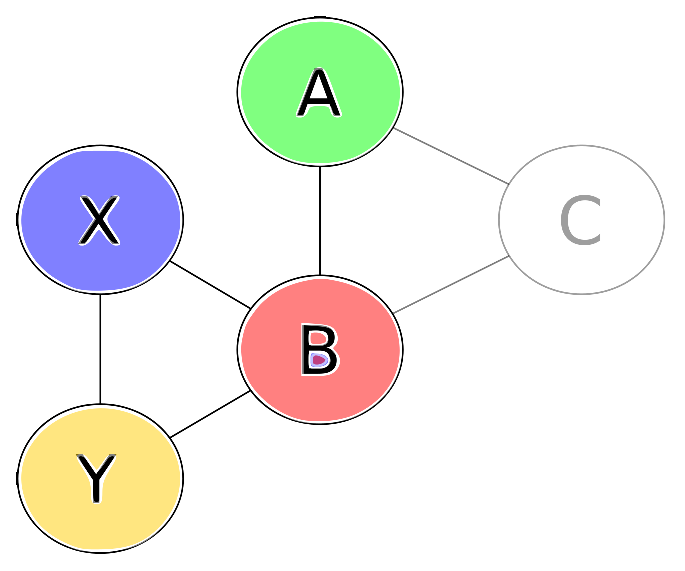
\includegraphics{img/eg_embed.eps}
		}
	\end{center}
	\caption[Embedding example]{The shape of an example Hamiltonian as would be created by \texttt{QCC}.  This graph will not fit on the \machine, so in the next section we will demonstrate the embedding algorithm on it.}
	\label{fig:eg_embed}
\end{figure}

\section{Embedding algorithm}
\label{sec:embed_algo}
Once we have our problem Hamiltonians we need to convert them into Hamiltonians which have the same shape as the graph that the \machine machine has.  This is done by adding \emph{clone spins} into the graph: each clone spin has the same value in the ground state as one of the logical spins in the input graph.  
This allows us to decrease the connectivity of the problem Hamiltonian until it is sparse enough to be the same shape as the physical machine.  The following algorithm is essentially equivalent to one presented in \cite{choi1}.
We expect that translating complete graphs onto graphs with constant connectivity to require roughly a quadratic size penalty in the number of clone spins (as the number of connections in a complete graph is $\sim n^2$).
Ideally, to ensure that each clone spin's ground state is the same as it's parent we would have $J_{ij} << J_{clone} \forall i,j$.  Because of physical limits of the machine (especially the resolution mentioned in Section \ref{sec:resolution}) large values of $J_{clone}$ may not maximize fidelity: for a machine with finite resolution, having a large $J_{clone}$ may compress other coupling values together such that the ground state starts to overlap with higher energy state.  On the other hand a too small value of $J_{clone}$ may result in ground states in which the clones are not aligned, which will almost certainly also produce incorrect ground states. Thus we have to find an empirical value of $J_{clone}$ that maximizes the fidelity while preserving the ground states.

\begin{figure}
	\begin{tabular}{l l l}
		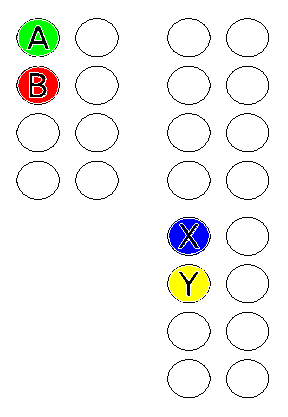
\includegraphics{img/eg_embed_full.eps} & \hspace{1 in} &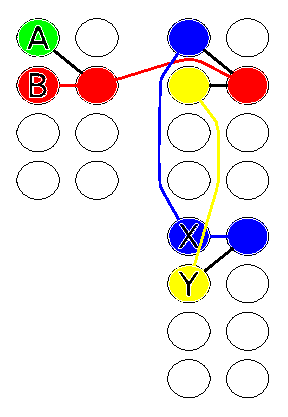
\includegraphics{img/eg_embed_full2.eps} \\
	\end{tabular}
	\caption[Embedding Algorithm]{This figure shows two steps in the embedding process.  On the left is the first step, assigning elements of the input graph (Figure \ref{fig:eg_embed}) along the diagonal of the \machine graph.  On the right is the connection step; nodes with the same colour share logical values.  Coloured lines represent the \emph{clone couplings}, while black lines represent the computational couplings.}
	\label{fig:embedding}
\end{figure}

Figure \ref{fig:embedding} shows a demonstration of the embedding algorithm.  The main idea is to assign nodes from the Hamiltonian you are trying to embed along the diagonal of the \machine graph.  Then link up connected nodes by cloning right and up from the nodes that need to be connected.

The embedding algorithm is as follows:

\emph{\textbf{Definitions:}}

Designate the input Hamiltonian graph $V$ and the output graph $G$.  Label the spins in $V$ and $G$ as $V_i$ and $G_i$ respectively.
We define the \emph{clone map} $C_i$ as the set of spins $[i,j \ldots]$ which have the same logical value as their parent spin: so for example the clone map of spin 5, $C_5$, might be $[2,3,13]$ which would mean that spins 2, 3, 5 and 13 all share the same logical value.  
We define a mapping $M$ between logical spins in graph $V$ and computation spins in graph $G$.  For example, spin $V_{12}$ representing the 12th variable in a problem might be mapped to $G_{187}$, the 187th machine spin.

We also define a \emph{clone coupling} value which is as large as possible and ferromagnetic; this attempts to ensure that all the members of a clone map are aligned in the ground state.  In the final $G$, each member of a clone map should have a clone coupling connecting it to at least one other member of the clone map.

\emph{\textbf{Procedure:}}
\begin{enumerate}
	\item Populate $M$ by mapping each $V_i$ to one of the spins $G_j$ on the left side of a unit cell that lies along the diagonal of $G$
	\item For each field term in $V$, add a field to $G$ on the corresponding spin
	\item For each $J_{ij}$ in $V$, conduct the following operation:
		\begin{itemize}
			\item Scan through both of $C_i$ and $C_j$ to find the pair which are nearest to each other in $G$; call these $x$ and $y$
			\item Get a list of each spin that lies along the path between $x$ and $y$
			\item Assign half of these spins to $C_i$ and half to $C_j$; add the appropriate clone coupling into $G$ for each spin in the path to ensure that the clone map is properly connected
			\item Finally, at the interface between the two new clone map members, add a coupling into $G$ with the same value as $J_{ij}$
		\end{itemize}
\end{enumerate}

Each term in $V$, both fields and couplings, should now have a corresponding term in $G$.  $G$ should also contain many coupling terms that group the necessary clone maps.  

This algorithm is tailored to AQC machines whose qubits are arranged in a square shape (specifically the shape of the \machine), however, the principle should be generalizable: as mentioned above any reasonably compact graph with constant connectivity should be able to embed a complete graph with an $n^2$ overhead by allocating the input graph spins along the diagonal.

\chapter{The \texttt{VESUVIUS} Machine}

\section{Resolution}
In addition to the graph-shape restrictions, the \texttt{VESUVIUS} machine cannot implement arbitrary physical Hamiltonians.  The machine can only implement fields and couplings as one of 15 distinct values: $-7/7, -6/7 \dots 5/7,6/7, 7/7$.  As our embedded Hamiltonians don't generally have these coupling values, they must be manipulated to fit in this range.
First we normalize all the field and coupling values into the range $[-1..1]$, and then coerce the coupling to the nearest machine implemented value.
Unfortunately we don't know exactly how the coercion is done; it seems reasonable that each normalized coupling would be rounded to the nearest machine implemented coupling, but other schemes such as rounding toward or away from zero are possible.

\chapter{Preliminary Results}
\label{chap:prelim}

\section{SAT-like Hamiltonian}
\begin{figure}[h]
	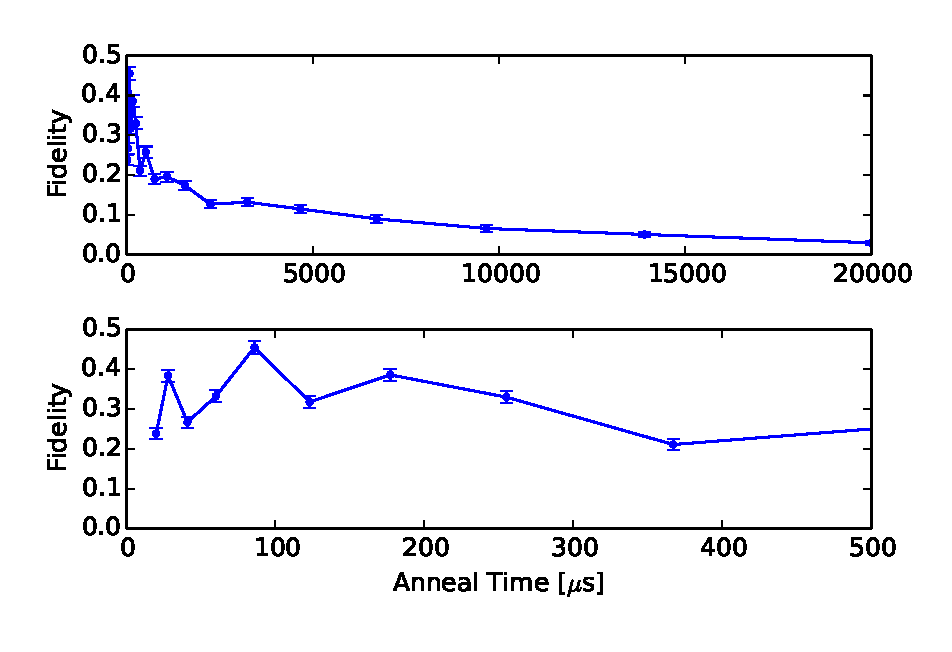
\includegraphics{img/6_018_2_fidelity.eps}
	\caption[Fidelity vs Time]{Plot of the fidelity as a function of annealing time for the Hamiltonian ``6\_018'' for both the full time range and the first 10 time points.  Both windows show the same data set.  Errors are estimated from $\sigma = \sqrt{np(1-p)}$.  Interesting features include the decrease in fidelity with longer anneal time and that the fidelity is very volatile over the short anneal time periods.}
	\label{fig:fidelity}
\end{figure}

Preliminary results were gathered on a sample quasi-random Hamiltonian called ``6\_018''.  This problem Hamiltonian was built up of clusters of clause sub-Hamiltonians in the same way as a SAT solver Hamiltonian would be, although ``6\_018'' does not encode a actual SAT problem.  This Hamiltonian was simple to generate and allowed us to verify our procedure for analyzing AQC results.
Data was collected in a series of evolutions at annealing times ranging from 20 $\mu$s to 20 ms.  Each evolution consists of choosing an anneal time and programming the problem Hamiltonian onto the hardware, then annealing 1000 times successively and reading out the final states.  We call each of these individual evaluations a \emph{read}, and a whole sequence of reads with the same programmed Hamiltonian a \emph{run}.  Any programming error (see \ref{sec:noise}) in the Hamiltonian should be the same between reads and differ between runs.

The state read out after each read is either the ground state, or some other higher energy (and incorrect) state.  The successes and failures thus follow a binomial distribution; there is some probability $p$ of getting the ground state, and probability $1-p$ of getting a different state.
Our best estimate of the fidelity from a single run is thus the fraction of successes, or $p = \frac{gs}{n}$ for $gs$ reads of the ground state and $n$ total reads.  We can also estimate the error in our estimate of the fidelity, because the variance of a binomial distribution is $\sigma^2 = np(1-p)$.

Figure \ref{fig:fidelity} shows the results of an initial set of runs spanning annealing times from 20 $\mu$s to 20 ms.  
There are several features of this data that stand out.  
First, contrary to our expectations, the fidelity \emph{decreases} as the anneal time increases.  We would expect that longer anneal times bring us closer to adiabatic evolution and thus remaining in the ground state.  This result suggests to us that adiabaticity (or lack thereof) is not dominating the fidelity for long annealing times. 
Second, there is significant change in the fidelity over very small changes in anneal time for less than $\sim 300$ $\mu$s, well outside what we would statistically expect based on the number of reads conducted.  This suggests that there is an uncontrolled factor besides the annealing time when the anneal time is short.  This factor disappears for longer anneal times, when whatever is damping the fidelity also seems to dampen the short time oscillations.

Figure \ref{fig:short_fidelity} shows the same data as in Figure \ref{fig:fidelity} as well as three more sweeps conducted in the same fashion, annealing out to 500 $\mu$s.  The large-short time oscillations are still seen, and of note is the fact that different runs of the same anneal time lie far outside their respective error margins.  This confirms our earlier suspicion that rather than the quantum annealing fidelity actually changing so rapidly with small changes in anneal time, there is some other uncontrolled factor which is changing from run to run.

\begin{figure}
	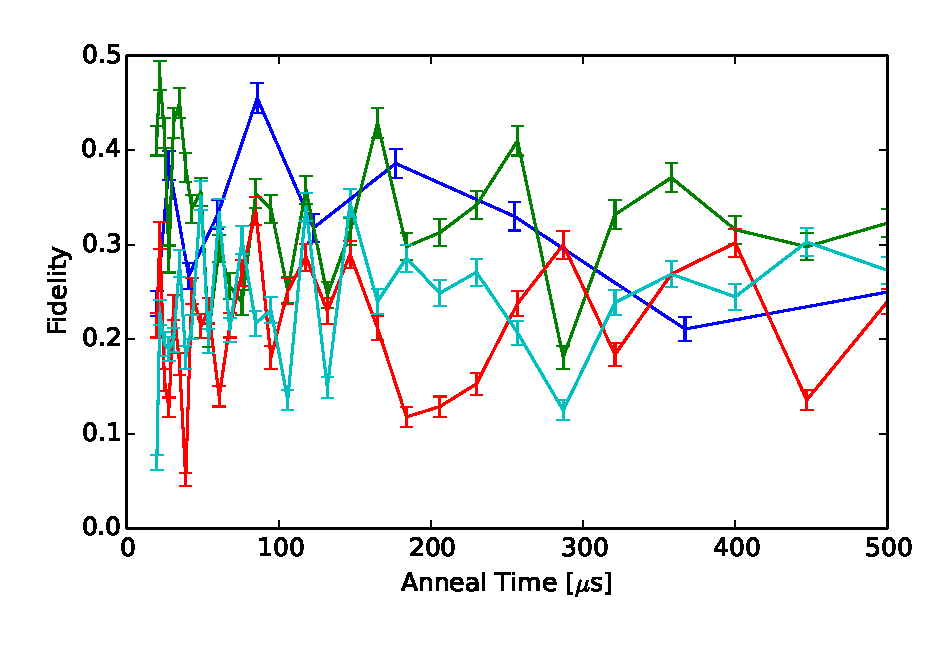
\includegraphics{img/6_018_comparison.eps}
	\caption[Short Time Fidelities]{The fidelity as a function of time for the Hamiltonian ``6\_018'' for several different machine runs.  Each data point consist of 1000 machine reads.  Notice the spread between machine runs is outside of the error bars.}
	\label{fig:short_fidelity}
\end{figure}

\section{Single Qubyte Hamiltonian}
The Hamiltonian shown in the above figures is large and reasonably complicated, with blocks of clauses and chains of clone spins spread across many qubytes.  Simplifying the Hamiltonian until we see smooth fidelity vs. time curves as we expect, and then increasing the complicating factors until we see the oscillations emerge would let us figure out what's causing them.  To that end a simple Hamiltonian consisting of a single qubyte of spins and encoding the logic of a single SAT clause was evaluated in the same fashion as the earlier ``6\_018'': runs at anneal times from 20 $\mu$s to 500 $\mu$s with 1000 reads per run.  

Figure \ref{fig:k44_comparison} shows the results of two such sweeps.  While the fidelity is higher than in the larger Hamiltonian's case, the short-time oscillations are still present.  The fidelity increase is in line with our expectations; as the number of spins grows the gap shrinks and fidelity drops for a given anneal time.  The continued presence of the short-time oscillations indicates that they're not simply a result of ``difficulty'' of the Hamiltonian (i.e. the gap or the problem size), but some other factor.

\begin{figure}
	\scalebox{0.50}{
		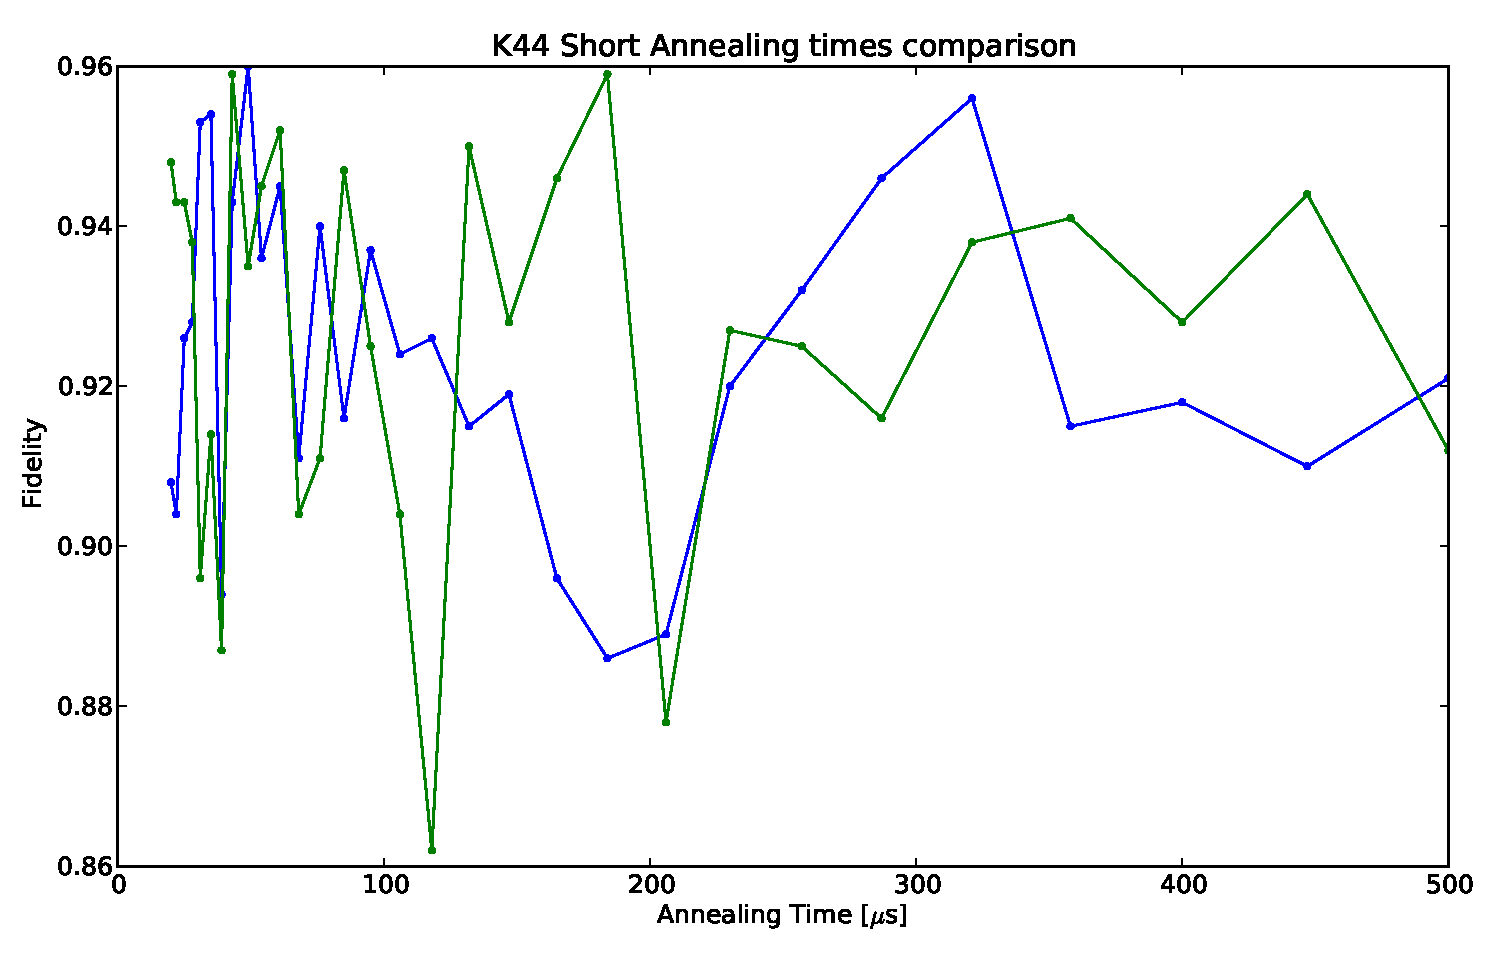
\includegraphics[bb= 0 0 600 400]{img/k44_comparison.pdf}
	}
	\caption[Single K44 Fidelity]{Fidelity as a function of anneal time for the Hamiltonian ``k44'' which consists of a single SAT clause embedded into a single qubyte.  The fidelity is higher than ``6\_018'' for the same anneal times, but the short-time oscillations are still present.}
	\label{fig:k44_comparison}
\end{figure}

\section{Boolean SAT Hamiltonian}

\chapter{Results and Discussion}
\begin{figure}
	\scalebox{0.4}{
		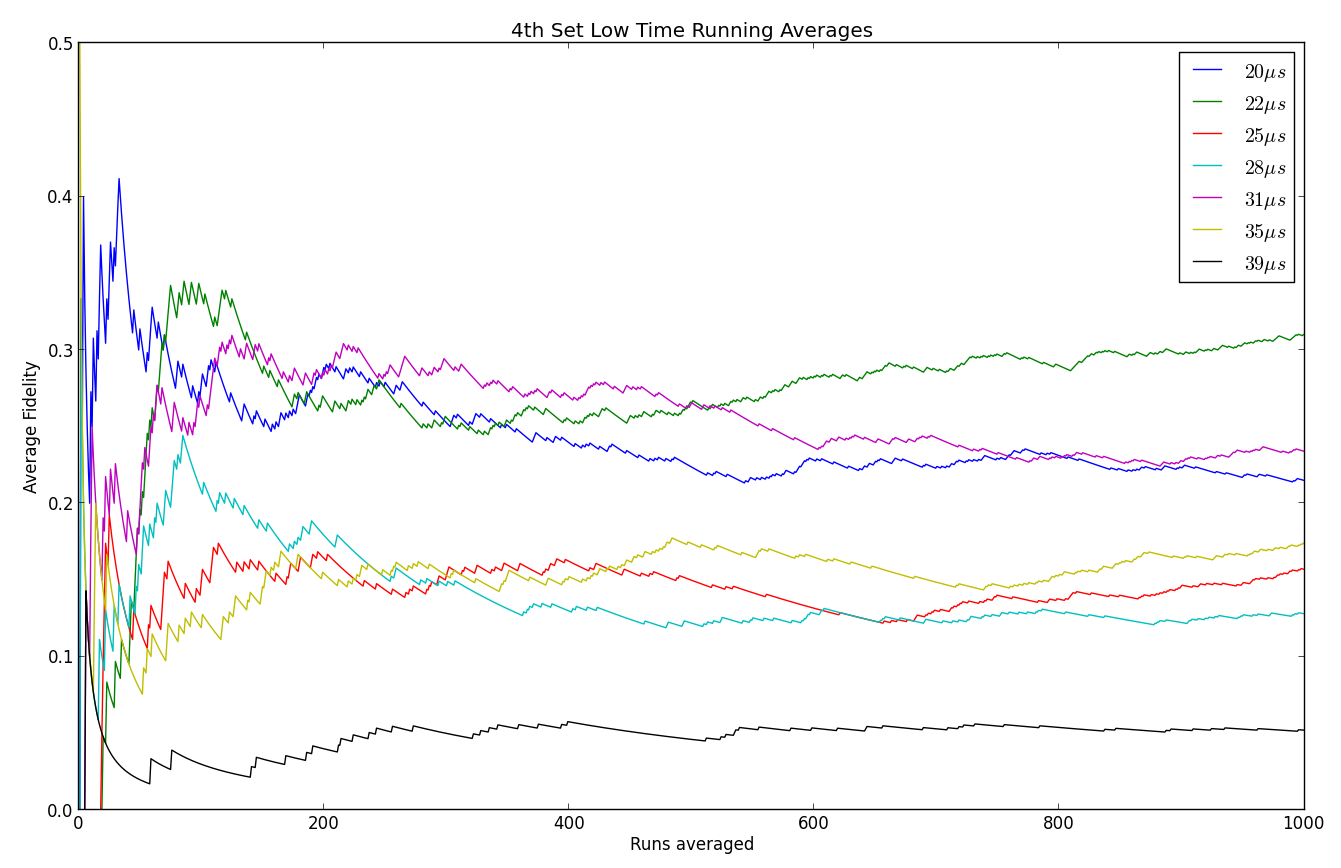
\includegraphics[bb= 0 0 1341 868]{img/4th_run_avg_low.png}
	}
	\caption[Running Fidelity Average]{Running average of the fidelity of the Hamiltonian ``6\_018'' for several short-time anneals, showing the change in fidelity with increasing read number.  The number of reads averaged over increases from zero to one thousand.  The rightmost edge of each data set shows the final fidelity estimate for that anneal time.  }
	\label{fig:running_avg}
\end{figure}
\section{Read noise}
First we examine the question of whether there is significant drift in the fidelity within a single run.  That is, does the probability of getting the ground state on any given read depend on the read number (the first read, second read etc.).  This question was examined on the Hamiltonian ``6\_018'' because the data collected on that particular Hamiltonian always consisted of at least 1000 reads per run.
Figure \ref{fig:running_avg} shows the running average of some short-time anneals from a single sweep of ``6\_018''.  If there is not significant read noise, we expect that the running average should flatten out and converge on the ``true'' fidelity after the appropriate number of reads.  For example, for a standard deviation $\sigma = \sqrt{np(1-p)}$ we expect that the running average should be within 5\% of the true fidelity after $\sim$ 200 reads.  Most of the anneal times appear to be reasonably flat past $\sim$ 500 reads, so the running averages appear to indicate to us that there isn't significant read noise (or at least, not nearly enough to be responsible for the short-time oscillations we saw in Chapter \ref{chap:prelim}).

The running average is a somewhat flawed quantity however, since it privileges earlier reads over later ones (since each read contributes like $1/N$ for $N$ reads already counted).  To remedy this we can also look at a rolling average of the fidelity as the reads come in.  Figure \ref{fig:rolling_avg} shows a rolling average of the fidelity for the same data as Figure \ref{fig:running_avg}.  Each point is the ground state fraction of the 100 reads around the labelled point; e.g. the value at point 500 is the number of ground states found from reads 450 to 550 over 100.  The rolling average has an advantage over the running average in that it does not prefer any part of the data set, but it can be harder to make out trends than in the running average.  It can be seen in the rolling average data that there does not appear to be a trend toward the fidelity being higher or lower in different segments of the run; e.g. the 22 $\mu$s run has highest fidelity in the nieghbourhood of read 600, while the 25 $\mu$s run has a minimum in the same location.

The combined results of the running and rolling averages would seem to indicate that intra-run errors, or errors occurring in the process of administering different reads, are not a significant contributor to the final observed fidelity for any given problem.

\begin{figure}
	\scalebox{0.35}{
		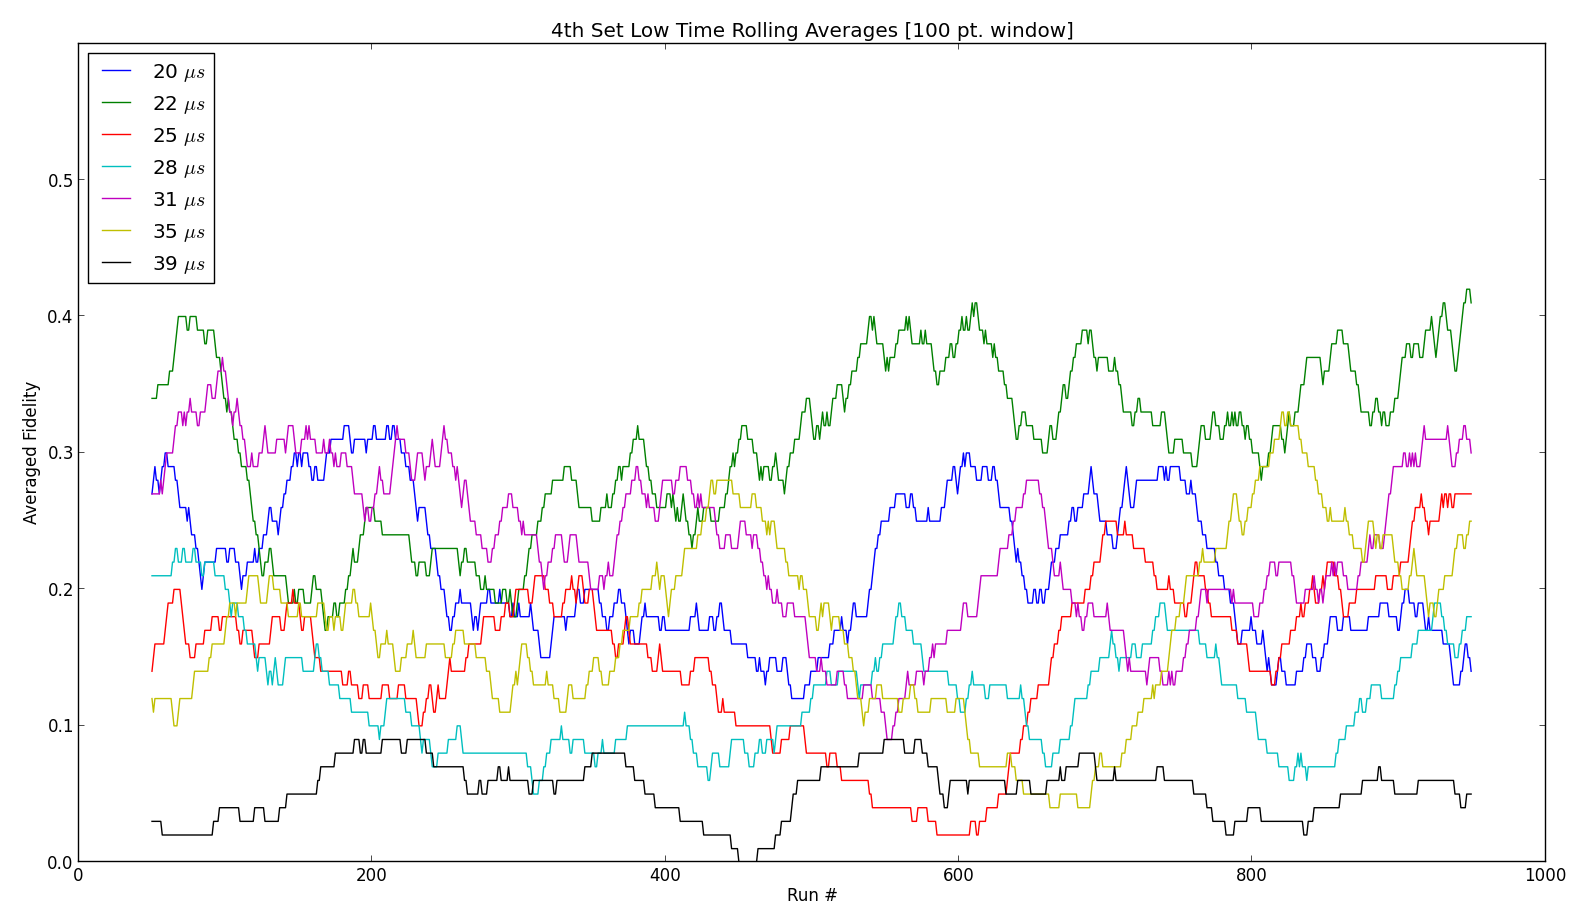
\includegraphics[bb=0 0 1582 917]{img/4th_run_roll_avg_low_100.png}
	}
	\caption[Rolling Fidelity Average]{Rolling average of the estimated fidelity for data collected from Hamiltonian ``6\_018'' at the seven shortest anneal times.  Each point is the average fidelity over a one hundred point window, e.g. the value at point 500 is the total number of times the ground state was measured between reads 450 and 550 divided by one hundred.}
	\label{fig:rolling_avg}
\end{figure}

\section{Short-time oscillations}
Looking to expand on the results of Chapter \ref{chap:prelim}, multiple sweeps of data were collected from a Hamiltonian labelled ``k44\_and''.  Figure \ref{fig:results_avg} shows the resulting fidelity estimates as a function of time.  This Hamiltonian not only occupies a single qubyte like ``k44'', but there is only one unique ground state.  These properties were chosen to attempt to minimize complicating factors.  Runs were carried out at annealing times from 20 $\mu$s to 20 ms as before.  Each run consisted of 100 reads, and 35 different runs were conducted at each anneal time.  Each fidelity estimate consists of a weighted average of each of the individual run estimates, weighted by the binomial error $\sigma$ for that run.
The error estimate at each anneal time is the standard deviation of the distribution of the individual run estimates.

Unlike in Chapter \ref{chap:prelim}, averaging over many runs at the same anneal time has managed to remove the short-time oscillations.  Figure \ref{fig:hist} shows a histogram of fidelities measured for ``k44\_and'' at an anneal time of 20 $\mu$s.  The Gaussian shape suggests that there are two effects going on: first, there is a value of the fidelity determined mainly by the quantum annealing (at the centre of the distribution) and second, that there is some noise applied over the fidelity from run to run.  The most likely source of this seems to be the programming error from imprecision of the physical couplings (see Sections \ref{sec:noise} and \ref{sec:coupling}).  If the noise in programming the couplings is high enough that if two adjacent couplings end up close enough together then the fidelity will drop because instead of the state we expect being the ground state and thus the most common, it will actually be some higher energy excited state and thus if the annealing is carried out successfully will have low probability of being found.  In the other scenario where two adjacent couplings are randomly bounced away from each other, it is entirely possible that in addition to the ground state being correctly encoded the gap is larger, thus increasing the fidelity.

\begin{figure}
	%includegraphics
	\caption[Averaged Anneal Results]{Fidelity vs anneal time with each data point averaged over multiple different runs.  Each run was used to estimate the fidelity independently as in Chapter \ref{chap:prelim}, with the final estimate the weighted average of each run.  The errorbars reflect the standard deviation of the distribution of estimates from each run.}
	\label{fig:results_avg}
\end{figure}

\begin{figure}
	%includegraphics
	\caption[Estimated Fidelity Histogram]{Histogram of the estimated fidelities for each run of the Hamiltonian ``k44\_and'' with an anneal time of 20 $\mu$s.  The shape appears roughly Gaussian, indicating that while there is a random factor in the fidelity that varies from run to run, there is still a central value that we take in this case to be roughly FIXME.}
	\label{fig:hist}
\end{figure}

\begin{figure}
	%includegraphics
	\caption[Fidelity Distribution vs. Time]{This figure shows the breadth of the distribution of estimated fidelities, i.e. the standard deviation $\sigma$ as a function of the annealing time for the Hamiltonian ``k44\_and''.  As the annealing time increases, the short-time oscillation effect observed in the preliminary results dies off and the distribution narrows.}
	\label{fig:std_time}
\end{figure}

Figure \ref{fig:std_time} shows the standard deviation of the fidelity estimates from evaluation of ``k44\_and'' as a function of the annealing time.  As we saw in the previous results, the large oscillations observed in the short-time fidelity die away as the annealing time increases.  This quantifies our earlier observation of the short-time oscillations: there are two regimes of the annealing, one below $\sim 500$ $\mu$s where the standard deviation is $\sim$ FIXME and one above $\sim 500$ $\mu$s where the standard deviation quickly drops down to FIXME.

This still does not explain \emph{why} the short-time oscillations do not persist into longer annealing times.  The above argument regarding overlap of the physical couplings applies just as well to annealing at longer times.

\section{Clone coupling value}
\label{sec:coupling}
As discussed in Sections \ref{sec:embed_algo} and \ref{sec:resolution}, while for an ideal machine maximizing the clone coupling value would ensure that adding clones did not alter the ground states of our problem Hamiltonians, the \texttt{VESUVIUS} machine can only implement 15 different clone coupling values.  In addition, these values must be evenly spaced.  If we were to use a clone coupling value of $-14$ in a problem Hamiltonian which natively had coupling values of $-2,-1,1,2$, this would result in compressing each of the positive and negative couplings into one machine value.  The machine only implements couplings of the form 
\begin{equation}
	\pm\frac{x}{7}, 1 \le x \le 7
\end{equation}
so the above example would result in a physically implemented Hamiltonian of $-1/7, -1/7, 1/7, 1/7$ in addition to the clone coupling of $-1$.  Most of the time this will result in a malformed Hamiltonian with incorrect ground states.

In addition to incorrect ground states, it is possible that the programming error in the machine is large enough to make the couplings $1/7$ and $2/7$ close enough to be likely to collide, whereas $1/7$ and $3/7$ could be far enough apart to be programmed correctly every time.  This could mean that even in scenarios where \texttt{VESUVIUS} has enough range to encode the problem Hamiltonian couplings correctly with a large clone coupling value we still don't want to do so.

This means that when selecting a clone coupling value we must balance these two competing factors, the desire to make the clone coupling as large as possible from a Hamiltonian correctness standpoint, and the desire to make it as small as possible from a machine resolution viewpoint.  The Hamiltonian correctness issue is correctness and knowable at the time the Hamiltonian is constructed; however in general to know whether a given clone coupling is large enough or not requires diagonalizing the Hamiltonian, and if this were possible then that would enable us to solve the initial computational problem directly.
The machine resolution problem is not necessarily the same from run to run; it could be that the compression of the problem Hamiltonian caused by the clone coupling value only makes it more likely for the machine to end up in an excited state.

To empirically examine the impact of the value of the clone coupling, the ``k44\_and'' Hamiltonian was embedded multiple different times with a clone coupling value ranging from -1 to -14 (from the smallest coupling in the problem Hamiltonian to twice the native resolution of the machine).  Figure \ref{fig:clone_coupling} shows the results of annealing these Hamiltonians from 20 $\mu$s to 20 ms.  Not only does fidelity increase as the clone coupling value is decreased, the short-time oscillations that we saw in Chapter \ref{chap:prelim} are removed.  At longer anneal times the difference in fidelity is reduced, and the same long-time drop in fidelities that was observed in other Hamiltonians continues.  This means that the mechanism for the long-time fidelity drop is not strongly impacted by the clone coupling value, which is what we would expect.

This provides more evidence that the short-time oscillations are caused by programming error in the \texttt{VESUVIUS} machine; if two couplings in the problem Hamiltonian are compressed together the correct ground states could still be formed in the resulting physical Hamiltonian if the couplings were randomly perturbed in the right directions, but this process would be random and differ greatly from run to run.

\begin{figure}
	%\includegraphics{}
	\caption[Variable Clone Coupling Fidelity]{The change in fidelity as the clone coupling value is scaled from -1 to -14.  The top view shows the scaling over the full time range 20 $\mu$s to 20 ms, while the bottom shows the same data zoomed in on the times 20 $\mu$s to 500 $\mu$s.  The fidelity increases with reducing clone coupling value, but using too small of a clone coupling value can result in incorrect ground states.}
	\label{fig:clone_coupling}
\end{figure}

\section{Size scaling}
The final property studied was the size scaling behaviour of the \texttt{VESUVIUS} machine.  This is 

\chapter{Conclusion}
A variety of Hamiltonians were constructed and evaluated on the \texttt{VESUVIUS} hardware.  We have seen several general methods for embedding problems into a form suitable for evaluation on an adiabatic quantum computer at a modest overhead, although even that overhead is a stiff price to pay on the current generation of adiabatic hardware.  Although the machine was not able to solve a 6 variable SAT problem, it was capable enough to solve several different toy problems.

In the process of solving these toy problems we discovered several factors important for using the D-Wave family of adiabatic machines.  Among them the fact that contrary to expectations shorter anneal times give better results, and that the limited number of built in machine couplings requires careful thought when embedding to ensure that coupling collisions do not occur.


\bibliographystyle{plain}
\bibliography{eskthesis}
\end{document}
